\section{lemma1}
Suppose we have a Riemann sphere $C$ and two diagrams $(C,\iota,\xi)$ and $(C,\iota',\xi')$ where they differ only in a small disk $D\subset C$. Let $D'$ be a slightly smaller co-centric disk inside $D$. Suppose there is a diffeomorphism between D and $\{(x,y)~|~x^2+y^2 < 4\}$ such that under this diffeomorphism 
\begin{itemize}
\item $D'$ is sent to $\{(x,y)~|~x^2+y^2 < 1\}$
\item the blue strand is sent to a strand that is isotopic to $\{(x,y)~|~y=\frac{1}{2}\}$($\{(x,y)~|~y = \frac{5}{3}x^2 - \frac{3}{4}\}$ resp.)
\item the red strand is sent to a strand that is isotopic to $\{(x,y)~|~y=-\frac{1}{2}\}$($\{(x,y)~|~y=\frac{1}{2}\}$ resp.)
\end{itemize}
Below figures show the diagrams on $D$.


\begin{figure}[H] % Optional: [h] means here, [t] for top, [b] for bottom, [p] for page of floats
    \centering
    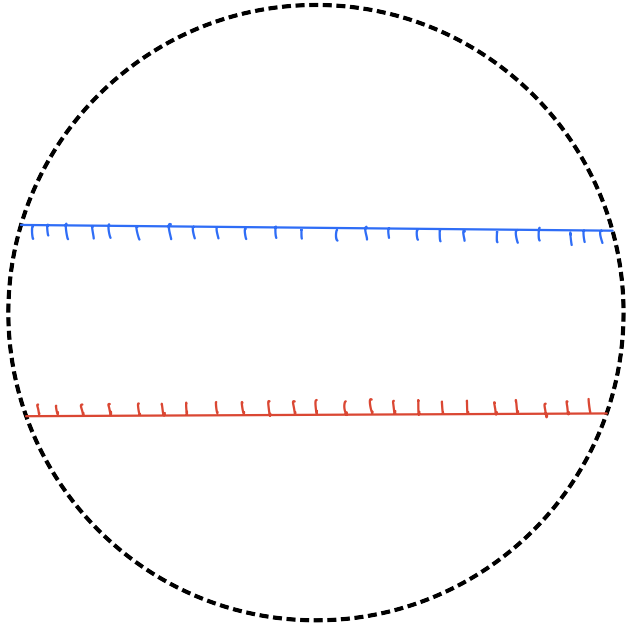
\includegraphics[scale = 0.95]{diagrams/lemma1/1.png} % Adjust the width as needed
    \caption{Your caption here}
    \label{fig:your-label}
\end{figure}


\begin{figure}[H] % Optional: [h] means here, [t] for top, [b] for bottom, [p] for page of floats
    \centering
    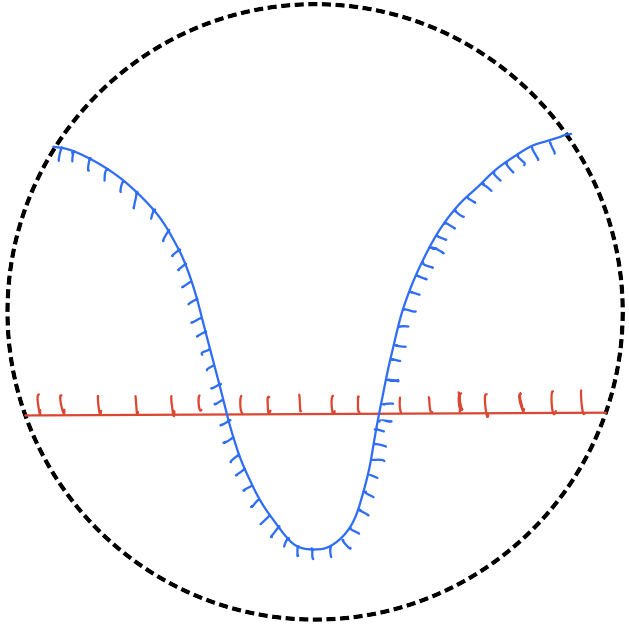
\includegraphics[scale = 0.95]{diagrams/lemma1/2.png} % Adjust the width as needed
    \caption{Your caption here}
    \label{fig:your-label}
\end{figure}

$isotopy_1$ defined in Definition1 defines an isotopy from $(C,\iota,\xi)$ to $(C,\iota',\xi')$. It defines a map $\mathcal{M}_{(C,\iota,\xi)}\rightarrow \mathcal{M}_{(C,\iota',\xi')}$. Under this map, a sheaf on $(C,\iota,\xi)$ described in the figure3 below is mapped to the sheaf on $(C,\iota',\xi')$ described in the figure4 below(figures below show only on $D$ where they differ because the stalks and generization maps away from the region remains the same).

\begin{figure}[H] % Optional: [h] means here, [t] for top, [b] for bottom, [p] for page of floats
    \centering
    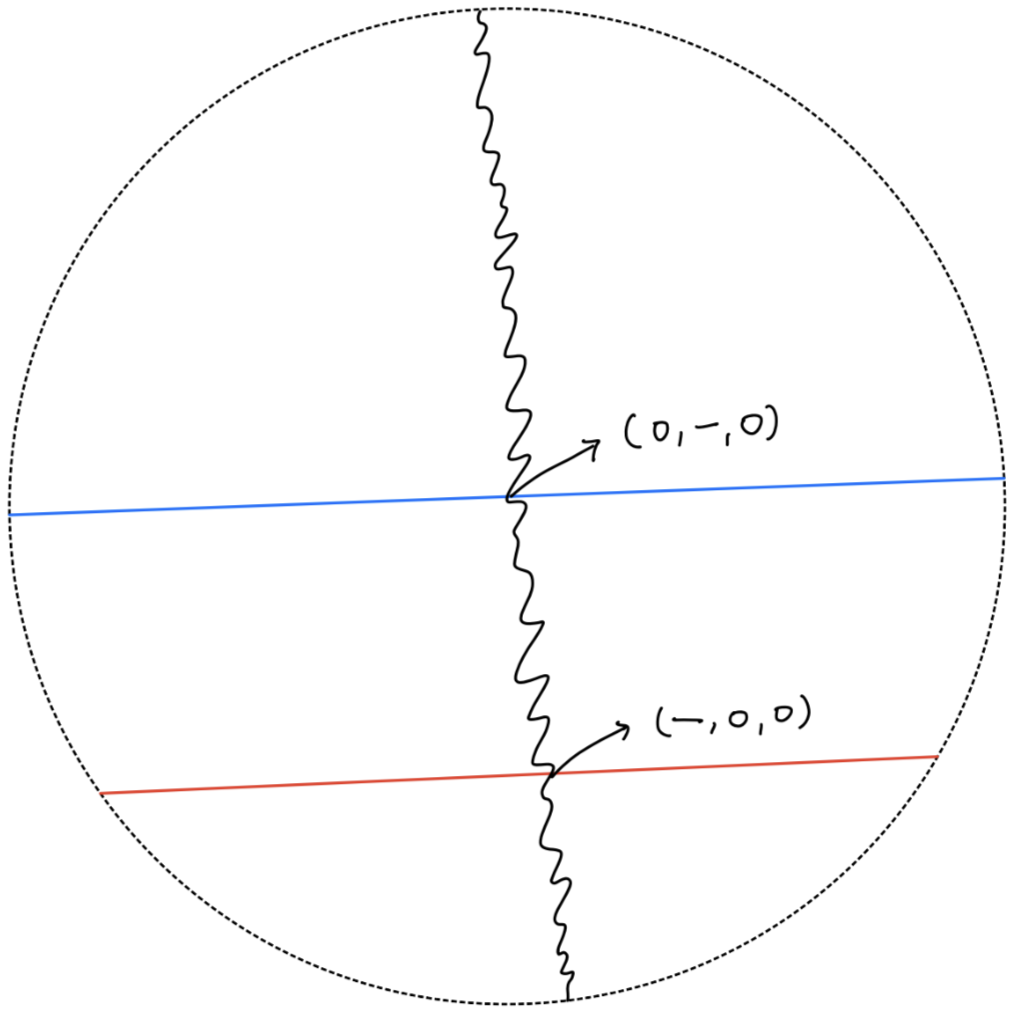
\includegraphics[scale = 0.95]{diagrams/lemma1/3.png} % Adjust the width as needed
    \caption{Your caption here}
    \label{fig:your-label}
\end{figure}
Stalks :
\begin{itemize}
\item $1$ : $\mathbb{C}^{m+1}$
\item $2$ : $\mathbb{C}^{m}$
\item $3$ : $\mathbb{C}^{m+1}$
\end{itemize}
Generization maps :
\begin{itemize}
\item $2\rightarrow 1$ : $\mathbb{C}^{m}\rightarrow \mathbb{C}^{m+1}$ where $e_i\mapsto e_{i+1}$
\item $2\rightarrow 3$ : $\mathbb{C}^{m}\rightarrow \mathbb{C}^{m+1}$ where $e_i\mapsto e_{i}$
\end{itemize}

\begin{figure}[H] % Optional: [h] means here, [t] for top, [b] for bottom, [p] for page of floats
    \centering
    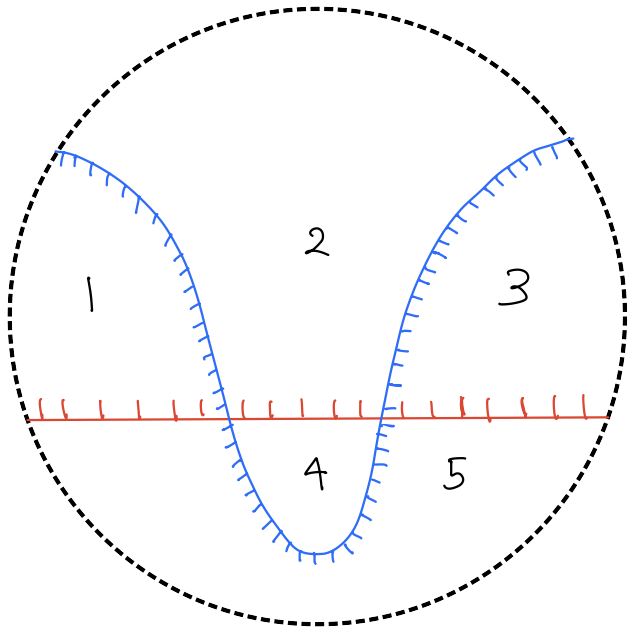
\includegraphics[scale = 0.95]{diagrams/lemma1/4.png} % Adjust the width as needed
    \caption{Your caption here}
    \label{fig:your-label}
\end{figure}

Stalks :
\begin{itemize}
\item $1$ : $\mathbb{C}^{m}$
\item $2$ : $\mathbb{C}^{m+1}$
\item $3$ : $\mathbb{C}^{m}$
\item $4$ : $\mathbb{C}^{m+2}$
\item $5$ : $\mathbb{C}^{m+1}$
\end{itemize}
Generization maps :
\begin{itemize}
\item $1\rightarrow 2$ : $\mathbb{C}^{m}\rightarrow \mathbb{C}^{m+1}$ where $e_i\mapsto e_{i+1}$
\item $3\rightarrow 2$ : $\mathbb{C}^{m}\rightarrow \mathbb{C}^{m+1}$ where $e_i\mapsto e_{i+1}$
\item $1\rightarrow 5$ : $\mathbb{C}^{m}\rightarrow \mathbb{C}^{m+1}$ where $e_i\mapsto e_{i}$
\item $3\rightarrow 5$ : $\mathbb{C}^{m}\rightarrow \mathbb{C}^{m+1}$ where $e_i\mapsto e_{i}$
\item $5\rightarrow 4$ : $\mathbb{C}^{m+1}\rightarrow \mathbb{C}^{m+2}$ where $e_i\mapsto e_{i+1}$
\item $2\rightarrow 4$ : $\mathbb{C}^{m+!}\rightarrow \mathbb{C}^{m+2}$ where $e_i\mapsto e_{i}$
\end{itemize}

(proof)